% !TeX spellcheck = en_GB

\section{Temporal Tuning Curves}
\label{sec:temporal_tuning_curves}

\begin{figure}
	\centering
	\includegraphics{media/chapters/04_temporal_tuning/temporal_responses_examples.pdf}%
	{\phantomsubcaption\label{fig:temporal_responses_examples_a}}%
	{\phantomsubcaption\label{fig:temporal_responses_examples_b}}%
	{\phantomsubcaption\label{fig:temporal_responses_examples_c}}%
	{\phantomsubcaption\label{fig:temporal_responses_examples_d}}%
	{\phantomsubcaption\label{fig:temporal_responses_examples_e}}%
	\caption[Illustration of possible in situ temporal response patterns]{Illustration of some possible \emph{in situ} temporal response patterns.
	\textbf{(A)} Neuron without pronounced temporal response.
	Pure tonic responses are relatively rare (e.g., Ruffini mechanoreceptors, cf.~\cite{kandel2012principles}, Figures~22-5~\&~23-9).
	\textbf{(B)} Neuron with a phasic response to a stimulus. Most sensory neurons are at least partially phasic (cf.~\cite{kandel2012principles}, Part~V).
	\textbf{(C)} Neuron which reaches its maximum firing rate $\theta$ seconds after the stimulus onset (e.g., time-cells, see below).
	\textbf{(D)} Neuron which oscillates rhythmically in response to a stimulus \citep[e.g.,][]{friedman-hill2000dynamics}.
	\textbf{(E)}~Neuron tuned to a specific temporal input pattern (see below).
	}
	\label{fig:temporal_responses_examples}
\end{figure}

Some neurons in the brain exhibit pronounced temporal activity patterns.
For example, as is illustrated in \Cref{fig:temporal_responses_examples}, their activities may extend beyond the stimulus period, cease before the stimulus has ended, repeat rhythmically, be tuned to specific spatiotemporal patterns, or any combination thereof.
Theoretical work suggests that diverse temporal responses form a representation of the past stimulus history \citep{grossberg1989neural,howard2014unified,voelker2018improving} and could, for example, support delay learning in the cerebellum (\cite{fujita1982adaptive,medina2000computer}; see also \Cref{chp:cerebellum}).
While spatiotemporal neural responses have originally been extensively studied in visual cortex \citep[e.g.,][]{deangelis1993spatiotemporal,carandini1999linearity}, more recent evidence indicates that various brain areas---including hippocampus, striatum, and cerebellum---possess neurons with pronounced temporal responses \citep[e.g.,][]{lusk2016cerebellar}.

In many cases, it is uncertain how these temporal response patterns come to be; that is, whether the temporal responses are a result of intrinsic neural properties, network-level effects, or a combination of both.
In this section, we build upon a linear filter model of temporal tuning \citep{watson1983look,adelson1985spatiotemporal} that is agnostic to these questions and that can be easily integrated into the \NEF as a generalisation of the dynamics principle.
We first review some types of temporal response patterns observed in biology, describe our extension to the \NEF, and then discuss examples of how this theory can be used in practice.

\subsection{Time Cells and Temporal Tuning}
\label{sec:temporal_tuning_biology}

\begin{figure}
	\centering
	\includegraphics{media/chapters/04_temporal_tuning/visual_cortex_tuning_spike_times.pdf}%
	{\phantomsubcaption\label{fig:visual_cortex_tuning_spike_times_a}}%
	{\phantomsubcaption\label{fig:visual_cortex_tuning_spike_times_b}}%
	\caption[Temporal properties of cells in visual cortex]{
		Temporal properties of cells in visual cortex.
		\textbf{(A)} Spike times from the Hubel and Wiesel experiment (same data as in \Cref{fig:visual_cortex_tuning}).
		The neuron is slightly phasic.
		Orange bar corresponds to the stimulus orientation.
		Adapted from \citet[Figure~3]{hubel1959receptive}.
		\textbf{(B)}~Illustration of a second-order high-pass filter. The step-response of such a filter (\emph{bottom}) could model the current flowing into the neuron, and thus the decaying activity.
	}
	\label{fig:visual_cortex_tuning_spike_times}
\end{figure}

Looking back at the data from the original experiment by \citeauthor{hubel1959receptive} (\citeyear{hubel1959receptive}; \Cref{fig:visual_cortex_tuning_spike_times_a}), as well as the temporal properties of other cortical sensory neurons \citep[cf.][Part~V]{kandel2012principles}, we find that these neurons tend to be \emph{phasic} (cf.~\Cref{fig:temporal_responses_examples_b}); that is, the observed spike rate decays after the stimulus onset.
Put differently, the neuron \emph{adapts} to the stimulus.

\subsubsection{Modelling phasic activity using high-pass filters}
As is depicted in \Cref{fig:visual_cortex_tuning_spike_times_b}, this activity profile could in principle be modelled by applying a high-pass filter to the neuron's somatic current.
For example, the impulse response $h(t)$ of a second-order high-pass filter can be constructed by subtracting two exponential low-pass filters with time-constants $\tau_1$, $\tau_2$:
\begin{align}
	h(t) &= \frac{1}{\tau_1} \exp\left( -\frac{t}{\tau_1} \right) - \frac{\alpha}{\tau_2} \exp\left( -\frac{t}{\tau_2} \right) \quad \text{for } t \geq 0 \,, \text{where } \alpha, \tau_1, \tau_2 > 0 \,, \text{and } \alpha \tau_1 < \tau_2 \,.
	\label{eqn:high_pass}
\end{align}

The idea behind \enquote{temporal tuning curves} (formalised below) is to treat $h(t)$ as a part of the neuron's tuning properties.
That is, we replace the encoder, or \enquote{preferred stimulus}, $\vec e$ with a temporal encoder $\vec{\mathfrak{e}}(t) = \vec{e} \cdot h(t)$, resulting in a \enquote{temporal preferred stimulus}.

Notably, in doing this, we do not subscribe to any specific mechanism that produces the high-pass characteristics.
In fact, this response pattern could be the result of intrinsic neural or synaptic dynamics, or instead stem form network-level effects.
As we discussed in \Cref{sec:neural_tuning}, this is one of the central ideas of a tuning curve---we characterise the behaviour of a neuron responding to an external stimulus \emph{in situ}, capturing both the computation performed by the network leading up to an individual neuron and the intrinsic properties of the neuron itself.
In the context of the Neural Engineering Framework, we would then use available neural resources to systematically realise these desired tuning properties.

\subsubsection{Time cells}

\begin{figure}
	\centering
	\includegraphics{media/chapters/04_temporal_tuning/time_cells_howard_tiganj_example.pdf}%
	{\phantomsubcaption\label{fig:time_cells_howard_tiganj_example_a}}%
	{\phantomsubcaption\label{fig:time_cells_howard_tiganj_example_b}}%
	{\phantomsubcaption\label{fig:time_cells_howard_tiganj_example_c}}%
	\caption[Illustration of time cells]{
		Illustration of time cells.
		The depicted simulation results (using the technique described by \cite{howard2014unified}) resemble the empirical data presented in \citet{tiganj2016sequential}.
		Lighter colours correspond to larger values.
		\textbf{(A)}~Normalised firing rate of $73$ simulated time cells with $\theta \in [\SI{0}{\second}, \SI{5}{\second}]$. Cells are sorted by the observed $\hat \theta$ (dotted line).
		Data obtained by feeding the impulse responses $h_\theta(t)$ depicted in \emph{(C)} into an ensemble of \LIF neurons with noisy somatic currents.
		\textbf{(B)}~Cosine-similarity between the activity vectors for each time-pair. The similarities spread out for larger $t$, making it harder to decode $t$.
		\textbf{(C)}~Impulse responses proposed by \citet{howard2014unified} for $\tau = \SI{0.1}{\second}$.
	}
	\label{fig:time_cells_howard_tiganj_example}
\end{figure}

A more interesting example of temporal response patterns are so-called \enquote{time cells}, first described by \citet{pastalkova2008internally} in rat hippocampus.
As is illustrated in \Cref{fig:temporal_responses_examples_c}, time cells reach their peak activity a certain time $\theta$ after the stimulus onset at $t_0$.%
\footnote{In the original \citet{pastalkova2008internally} experiment, the \enquote{stimulus onset} corresponds to the animal beginning to perform some behavioural task, namely running in a wheel.}
This delay $\theta$ is specific to each cell and can be in the millisecond to seconds range.
Populations of time cells encode the time since the stimulus onset $t - t_0$, or, assuming continuous input signals, a compressed version of the stimulus history.
We discuss this in more detail below in \Cref{sec:temporal_bases}.

Time cells have also been described in other brain regions, including medial prefrontal cortex (\cite{tiganj2016sequential}), striatum, and the cerebellum (see \cite{lusk2016cerebellar} for a review).
Qualitatively, the normalised neural activities resemble the data depicted in \Cref{fig:time_cells_howard_tiganj_example_a}.
As time progresses, the population activities tend to become more similar (\Cref{fig:time_cells_howard_tiganj_example_b}).

\citet{howard2014unified} propose the following impulse response $h_\theta(t)$ (cf.~\Cref{fig:time_cells_howard_tiganj_example_c}) that can be approximated as a weighted sum of first-order low-pass filters:
\begin{align*}
	h_\theta(t)
	&=
		\alpha_\theta t^{\frac{\theta}{\tau}} e^{-\frac{t}{\tau}}
	\approx
		\sum_{i = 1}^q w_i e^{-\frac{t}{\tau_i}}
	\quad \text{for } t \geq 0 \text{ and where } \alpha_\theta \text{ is such that } \int_{0}^\infty h_\theta(t) \,dt = 1 \,.
\end{align*}
This model is biologically plausible, qualitatively reproduces empirical data, and has been proposed as a model for spatial representations in hippocampus as well.
Still, as we discuss below, there are theoretical reasons why relying on linear combinations of exponential filters can be suboptimal.
\Citet{voelker2018improving} demonstrate that the recurrent Legendre Delay Network (\LDN) similarly reproduces time cell data (see \Cref{sec:spiking_temporal_bases}).

\subsubsection{Space-time receptive fields in visual cortex}

\begin{figure}
	\centering
	\includegraphics{media/chapters/04_temporal_tuning/space_time_receptive_field.pdf}%
	{\phantomsubcaption\label{fig:space_time_receptive_field_a}}%
	{\phantomsubcaption\label{fig:space_time_receptive_field_b}}%
	{\phantomsubcaption\label{fig:space_time_receptive_field_c}}%
	\caption[Example of a space-time receptive field tuned to downwards motion]{Example of a space-time receptive field $\mathfrak{e}(t; \xi_1, \xi_2)$ tuned to downwards motion. The field is a Gabor filter (cf.~\Cref{sec:neural_tuning}) with shifting phase and exponential decay.
	\textbf{(A, B)} Different slices through $\mathfrak{e}$.
	Blue corresponds to positive, red to negative values.
	\textbf{(C)} Computing the neural activity for a grating pattern $\mathfrak{x}$ moving in the arrow direction.
	Line styles encode the pattern velocity (cf.~diagonal lines in \emph{(A)} for vertical motion); the solid line is matched to the velocity of the receptive field.
	Downwards motion results in the strongest response.
	Oscillatory behaviour encodes the phase.
	}
	\label{fig:space_time_receptive_field}
\end{figure}

Linear models of simple cells in visual cortex were our main motivation for modelling tuning curves in the \NEF as the dot-product between the stimulus $\vec x$ and a normalised encoder $\vec e$ (cf.~\Cref{sec:neural_tuning}).
Similarly, linear models of the temporal behaviour of simple cells---beyond the previously discussed phasic response---serve as our basis for extending the \NEF toward temporal tuning.

The basic observation is that some cells in visual cortex reach their maximum firing rate for specific stimulus signals.
For example, some cells only react to edges moving in a certain direction at a specific velocity.
%Historically, models of these directionality effects relied on nonlinear interactions in small model circuits \citep[e.g.,][]{emerson1977simple}.
%Theoretical work by \citet{watson1983look,adelson1985spatiotemporal} suggested that neural activity could instead be modelled linearly.
One possible way to construct a model of this spatiotemporal tuning is to use a \emph{space-time receptive field} $\mathfrak{e}(t; \xi_1, \xi_2)$, where $\xi_1$ and $\xi_2$ are coordinates in the visual field and $t \geq 0$ is time (\cite{watson1983look,adelson1985spatiotemporal}; see \cite{carandini1999linearity}, for a review).
Given stimulus history $\mathfrak{x}(t; \xi_1, \xi_2)$, the neural activity $a(\mathfrak{x})$ at $t = 0$ can be modelled by convolving over the instantaneous inner products between $\mathfrak{x}$ and $\mathfrak{e}$.
Borrowing the gain and bias terms $\alpha$, $\beta$, as well as the response curve $G$ from the \NEF, we have
\begin{align}
	a(\mathfrak{x})
		&= G\left[\alpha \! \iiint_0^\infty \!\!\! \mathfrak{e}(\tau; \xi_1, \xi_2) \, \mathfrak{x}(-\tau; \xi_1, \xi_2) \,
		\D \tau \D \xi_1 \D \xi_2 + \beta \right]
		 = G\left[\alpha \! \int_0^\infty \!\!\! \big\langle \mathfrak{e}(\tau), \mathfrak{x}(-\tau) \big\rangle \,
		\D \tau + \beta \right] \, .
	\label{eqn:tuning_curve_from_temporal_receptive_field}
\end{align}

The space-time receptive fields of individual neurons (sometimes referred to as \enquote{weighting functions}) can be reconstructed by exposing animals to computer generated imagery \citep{mclean1989contribution}.
An example of an artificial space-time recepitve field that qualitatively resembles empirical data \citep[cf.][]{deangelis1993spatiotemporal} is depicted in \Cref{fig:space_time_receptive_field}.

\subsection{Temporal Tuning Curves and the Neural Engineering Framework}
\label{sec:temporal_tuning_nef}

The above summary of biological temporal response patterns provides some motivation as for why modelling temporal tuning can be desirable.
We now define this concept more rigorously, and, in the next subsection, compare it to the original \NEF dynamics principle.

The most general definition of a \enquote{temporal tuning curve} is \enquote{a function that maps the past history of a $d$-dimensional stimulus onto the average expected activation of a neuron}.

\begin{definition}
	\label{def:temporal_tuning_curve}
	A \emph{temporal tuning curve} $a(\vec{\mathfrak{x}})$ is a second-order function mapping from the past stimulus history $\mathfrak{x}$ onto the average neural activity at $t = 0$ (i.e., the present).
	In other words, $a : (\mathbb{R}^- \longrightarrow \mathbb{R}^d) \longrightarrow \mathbb{R}$, where $\mathbb{R}^- = \{ x \mid x \in \mathbb{R} \text{ and } x \leq 0 \}$.
\end{definition}

Of course, this definition includes a wide range of imaginable functions and is thus not very practical.
One particular class of temporal tuning curves that fits the \NEF well are \enquote{linear temporal tuning curves}, inspired by the space-time receptive fields discussed above.

\begin{definition}
	\label{def:linear_temporal_tuning}
	\emph{Linear temporal tuning curves} are a special class of temporal tuning curves.
	Let $G[J]$ be a neural response curve, then the average activity of the $i$th post neuron is modelled as
	\begin{align}
		a_i(\vec{\mathfrak{x}})
			= G\left[ J_i \left( \int_{0}^\infty \!\!\! \big\langle \vec{\mathfrak{e}}_i(\tau), \vec{\mathfrak{x}}(-\tau) \big\rangle 	\,\mathrm{d}\tau \right) \right]
		= G\left[ \alpha_i \! \int_{0}^\infty \!\!\! \big\langle \vec{\mathfrak{e}}_i(\tau), \vec{\mathfrak{x}}(-\tau) \big\rangle \,\mathrm{d}\tau + \beta_i \right] \,,
		\label{eqn:temporal_tuning_curve}
	\end{align}
	where the \emph{temporal encoder} $\vec{\mathfrak{e}}_i$ is a function $\vec{\mathfrak{e}}_i : \mathbb{R}^+ \longrightarrow \mathbb{R}^d$ over time.
	%The temporal encoder describes both an impulse response and a spatial receptive field.
\end{definition}
\noindent Limiting the temporal encoder to nonnegative times ensures that $\vec{\mathfrak{e}}_i$ is a causal filter.
As before, we assume that the current translation function $J_i(\xi)$ is affine with gain $\alpha_i$ and bias~$\beta_i$.

As with standard tuning-curves, \cref{eqn:temporal_tuning_curve} is a \emph{normative constraint} (cf.~\Cref{sec:nef_representation}).
However, in addition to what we had before, the temporal encoder $\vec{\mathfrak{e}}_i$ allows modellers to define some desired \emph{dynamics}.
This effectively unifies the \NEF dynamics and representation principles; as we discuss below, the weight solver can draw upon the dynamics of the pre-population as well as temporal resources such as synaptic filters to approximate the desired dynamics.

\subsubsection{Normalisation and preferred temporal stimuli}
In many cases, it may be useful to normalise the magnitude of the temporal encoder to an integral of one over time:
\begin{align}
	\int_{0}^\infty \| \vec{\mathfrak{e}}(\tau) \| \,\D \tau &= 1 \,.
	\label{eqn:normalisation}
\end{align}
In this way, and with some squinting, the temporal encoder can be interpreted as a \emph{preferred temporal stimulus}.
Note that normalisation is not possible for temporal encoders with an infinite energy, such as oscillators and integrator dynamics without decay.%
\footnote{Both the signal $\vec{\mathfrak{x}}$ and the encoder $\vec{\mathfrak{e}}$ must be normalised for the convolution between the encoder and the stimulus to correspond to a cosine similarity.
However, given its unbounded nature, it is unclear how the signal history $\vec{\mathfrak{x}}$ should be normalised.
Essentially, we would have to normalise with respect to some window function.}

\subsubsection{Synaptic filters as temporal encoders}
We can easily confirm that our notion of temporal tuning is compatible with the standard \NEF population dynamics.
Remember from \Cref{sec:nef_dynamics} that we typically assume a linear synaptic filter $h$.
Correspondingly, given some time-invariant normalised encoding vector $\vec e_i$, and assuming that the synapses are modelled as a first-order low-pass filter, a population naturally posses the following temporal encoder
\begin{align}
	\vec{\mathfrak{e}}_i(t)
		&= h(t) \vec e_i \,, & \text{with } h(t) &= \tau^{-1} \exp(-t \tau^{-1}) & \text{for } t > 0 \,.
	\label{eqn:synaptic_filter}
\end{align}
This temporal encoder fulfils the normalisation constraint in \cref{eqn:normalisation}.
Furthermore, as one would expect, combining \cref{eqn:synaptic_filter} and \cref{eqn:temporal_tuning_curve} yields the standard \NEF population dynamics:
\begin{align}
	a_i(\vec{\mathfrak{x}})
		&= G\left[ \alpha_i \! \int_{0}^\infty \!\!\! \big\langle h(\tau) \vec{e}_i, \vec{\mathfrak{x}}(-\tau) \big\rangle \,\mathit{d\tau} + \beta_i \right]
		 = G\left[ \alpha_i \big\langle \vec e_i, (\vec{\mathfrak{x}} \ast h)(0) \big\rangle + \beta_i \right] \,.
	\label{eqn:synaptic_filter_tuning_curve}
\end{align}

Importantly, this does not imply that the temporal encoder is in any way defined by the synaptic filter $h$; modellers can still choose any $\mathfrak{e}_i$ they desire.
However, unless there are other temporal resources in the network---such as diverse temporal tuning of the pre-population or recurrent connections, these are the only dynamics that can be well approximated.
%Notwithstanding neural dynamics, the \emph{intrinsic} temporal tuning of neuron population without recurrent connections just happens to be its synaptic filter.

%The point of temporal tuning curves, and, to some degree, the NEF dynamics principle, is that we can exploit the existing synaptic filters $h$, as well as neural dynamics as a \enquote{temporal resource} that can be exploited to form more complex dynamics.

\subsubsection{General weight optimisation problem}
Naturally, this raises the question of how to ensure that a pre-population possesses diverse temporal tuning.
While we could try to manually diversify synaptic filters, remember that one of the fundamental ideas of the \NEF is to specify tuning as a normative constraint, and to solve for connection weights that realise this tuning.

To this end, we propose a temporal variant of the current-space least-squares loss from \Cref{sec:nef_extension}.
If so desired, we can combine this loss function with subthreshold relaxation (\Cref{sec:nef_subthreshold}), nonnegativity constraints (\Cref{sec:nef_nonneg}), and dendritic nonlinearities (\Cref{sec:nef_nonlinear}).

As a first step, consider the loss function for connecting two neuron populations representing $d$-dimensional quantities without any transformation $f$.
Both neuron populations will represent the same quantity, but with potentially different temporal tuning.

Let $a_j(\mathfrak{x})$ be the temporal tuning curve of the $j$th pre-neuron, $J_i$ the current-translation function, and $h_{ij}$ the synaptic filter between the $j$th pre- and $i$th post neuron; this may include axonal and synaptic transmission delays.
Furthermore, let $N$ be the number of input signals (i.e., samples), and $m$ the number of pre-population neurons.
We have
\begin{align}
	E &= \sum_{k = 1}^N \left[
		J_i \left( \! \int_0^\infty \!\!\! \big\langle \mathfrak{e}_i(\tau), \mathfrak{x}_k(-\tau) \big\rangle \, \mathit{d\tau} \right) \,\,-\,\,
		\sum_{j = 1}^m w_{ij} \! \int_0^\infty \!\!\! h_{ij}(\tau) a_j(\mathfrak{x}_k \ast \delta_\tau) \,\mathrm{d}\tau
	\right]^2 \,,
	\label{eqn:weight_optimise_currents_temporal_no_trafo}
\end{align}
where $\delta_{\theta}(t) = \delta(t - \theta)$ is a shifted Dirac delta.
Correspondingly $(\mathfrak{x}_k \ast \delta_{\theta})(t) = \mathfrak{x}_k(t - \theta)$, and so $a_j(\mathfrak{x}_k \ast \delta_\tau)$ is the activity of the $j$th pre-neuron at time $-\tau$.

The term before the minus sign in \cref{eqn:weight_optimise_currents_temporal_no_trafo} is the current required to obtain our desired temporal tuning from \cref{eqn:temporal_tuning_curve}; the term after the minus sign uses the pre-population temporal tuning and the synaptic filters as a \emph{spatiotemporal function basis} to decode the desired currents.
While we know that randomly choosing spatial encoders $\vec e_j$ results in diverse \emph{spatial} pre-population tuning (\Cref{sec:dendritic_computation_theory}), we discuss in \Cref{sec:temporal_bases} how this basis can be made as \emph{temporally} diverse as possible.
Note that our optimisation problem is similar in principle to optimal Wiener filters \citep[Chapter~2]{wiener1949extrapolation,haykin2014adaptive}.
We discuss this in more detail in the context of \emph{adaptive} filters in \Cref{sec:adaptive_filter} and \Cref{chp:cerebellum}.

Lastly, note that our loss function is \emph{not} an integral over time---as is for example common in optimal control theory \citep[e.g.,][Chapter~14]{brogan1991modern}.
Instead, we take advantage of the fact that our temporal tuning curves are defined as the average activity of the neuron in the \emph{present}, i.e., at time $t = 0$.
Correspondingly, we only minimise the error at a single point in time, namely $t = 0$, but for a large set of input samples $\mathfrak{x}_k$.
We can thus tabulate \cref{eqn:weight_optimise_currents_temporal_no_trafo} as
\begin{align*}
	\vec w_i = \arg\min_{\vec w_i} \| \mat A_i \vec w_i - \vec J_i \|_2^2 \quad\quad \Rightarrow \quad\quad \vec w_i = \mat A_i^+ \vec J_i \,, \quad\quad \text{where} \quad \mat A_i \in \mathbb{R}^{N \times m}, \quad \vec J_i \in \mathbb{R}^n \,,
\end{align*}
and where $\mat A_i^+$ is the Moore-Penrose pseudo-inverse.
Put differently, and assuming that $\mathfrak{x}_k$ is finite and that all quantities have been appropriately sampled, minimising \cref{eqn:weight_optimise_currents_temporal_no_trafo} is the same kind of convex optimisation problem previously encountered in \Cref{sec:nef_extension}.

The primary challenge in solving this optimisation problem lies in selecting suitable input signals $\mathfrak{x}_k$ \citep[cf.][Section~10.2.5]{verhaegen2007filtering}---we discuss this in more detail in \Cref{sec:solve_dynamics_nonlinear_neurons}.
Choosing $\mathfrak{x}_k$ is particularly important if the desired tuning cannot be realised precisely; the frequency content of the training signals then determines the regime over which the approximation works well.
In our examples we use low-pass filtered white noise as $\mathfrak{x}_k$.

Finally, consider the case where we additionally solve for a spatiotemporal transformation, that is, a function $f$ that maps from a $d$-dimensional signal $\mathfrak{x}$ onto a $d'$-dimensional quantity, i.e., $f : (\mathbb{R}^- \longrightarrow \mathbb{R}^d) \longrightarrow \mathbb{R}^{d'}$ (cf.~\Cref{tbl:spatiotemporal}; see \Cref{sec:spatiotemporal} for examples).
We have:
\begin{align}
	E &= \sum_{k = 1}^N \left[
		J_i \left( \! \int_0^\infty \!\!\! \big\langle \mathfrak{e}_i(\tau), f(\mathfrak{x}_k \ast \delta_\tau) \big\rangle \, \mathit{d\tau} \right) \,\,-\,\,
		\sum_{j = 1}^m w_{ij} \! \int_0^\infty \!\!\! h_{ij}(\tau) a_j(\mathfrak{x}_k \ast \delta_\tau) \,\mathrm{d}\tau
	\right]^2 \,.
	\label{eqn:weight_optimise_currents_temporal}
\end{align}
As we explain in far more detail below, this equation unifies the \NEF representation, transformation, and dynamics principles.
To summarise:
\begin{enumerate}[1.]
	\item \emph{Representation.} To find identity decoders $\mat D_{\theta'}$, use \cref{eqn:weight_optimise_currents_temporal_no_trafo}.
	Set $J_i(\xi) = \xi$ and $\mathfrak{e}_i = (\mat I)_i \delta(-\theta')$.
	Choosing $\theta' < 0$ queries information present in the neuron population about the past.
	\item \emph{Transformation.} Directly use \cref{eqn:weight_optimise_currents_temporal}; we can compute function decoders $\mat D^f$ as above.
	\item \emph{Dynamics.} To realise linear dynamics, choose $\mathfrak{e}_i(t) = \langle \vec e^\mathrm{t}_i, \exp(\mat A t) \mat B \rangle$ where $\vec e^\mathrm{t}_i \in \mathbb{R}^{q}$.\footnote{As mentioned in the introduction, realising nonlinear dynamics is technically possible, but notationally inelegant. We would have to rely on the general definition of temporal tuning (\Cref{def:temporal_tuning_curve}) and solve for $G_i^{-1}[a_i(\mathfrak x_k)]$.
	Also, note that realising nonlinear dynamics is less important than it may seem; we can decode arbitrary nonlinear spatiotemporal $f$ from neurons with linear tuning due to the nonlinear response curve $G_i$.
	}
\end{enumerate}

\pagebreak

\subsection{Implementing Linear Time-Invariant Systems}
\label{sec:temporal_tuning_lti}

For the sake of simplicity, we first focus on linear networks and dynamical systems.
In particular, we discuss realising linear time-invariant (\LTI) systems in networks with linear response curves and current-translation (i.e., $G_i[J] = J$ and $J_i(\xi) = \xi$).
Essentially, each \enquote{neuron} corresponds to a separate represented dimension.

This restriction is less severe than it may seem.
\LTI systems are quite useful, and we can use the \NEF representation and transformation principles (\Cref{sec:nef_representation,sec:nef_transformation}) to emulate linear networks with nonlinear neurons.
Still, we discuss examples with more complex nonlinear networks and dynamics in \Cref{sec:recurrent_weights}.

\subsubsection{Feed-forward dynamics}

\begin{figure}
	\centering
	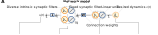
\includegraphics{media/chapters/04_temporal_tuning/feed_forward_dynamics.pdf}\\[-0.875em]
	\includegraphics{media/chapters/04_temporal_tuning/feed_forward_dynamics_plots.pdf}
	\caption[Solving for desired dynamics in a feed-forward linear network]{Solving for desired dynamics in a feed-forward linear network.
	\textbf{(A)} Overview of the network architecture. 
	A collection of $q$ synaptic filters diversifies the temporal response in a pre-population.
	%Due to linearity of the network, we can move the connection weight matrix $\mat B$ past the post-population.
	\textbf{(B, C, D, E)}~Example with $q = 4$ first-order low-pass filters (time-constants $\SI{10}{\milli\second}$, $\SI{22}{\milli\second}$, $\SI{46}{\milli\second}$, and $\SI{100}{\milli\second}$).
	The desired dynamics are a high-pass filter (eq.~\ref{eqn:high_pass}, $\tau_1 = \SI{20}{\milli\second}$, $\tau_2 = \SI{40}{\milli\second}$, $\alpha = 1$).
	\emph{Top:} System response to a band-limited white noise signal $u(t)$.
	\emph{Bottom:} Impulse response.
	Dotted line in \emph{(E)} is the desired response, solid line is the response when solving for $\mat{W}$ using least-squares.
	}
	\label{fig:feed_forward_dynamics}
\end{figure}

Assume that a pre-population possesses diverse temporal tuning.
We can now use \cref{eqn:weight_optimise_currents_temporal} to solve for desired post-population dynamics in feed-forward networks.
This is possible because the diverse temporal tuning of the pre-neurons forms a \emph{temporal basis}---just like the time-invariant tuning of an \NEF population forms a basis from which arbitrary functions $f$ can be decoded (cf.~\Cref{fig:nef_transformation}).

\Cref{fig:feed_forward_dynamics} provides an example of this concept.
Each pre-population neuron possesses a slightly different synaptic filter time-constant, and we solve for weights that result in high-pass filter tuning of the post-population.
This is the same idea as in the time-cell model by \citet{howard2014unified}, although we take the synaptic filter of the post-population into account as well.

\begin{figure}[p]
	\centering
	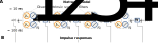
\includegraphics{media/chapters/04_temporal_tuning/feed_forward_low_pass_network.pdf}
	\includegraphics{media/chapters/04_temporal_tuning/feed_forward_low_pass.pdf}
	\caption[Chaining populations with diverse temporal tuning]{Chaining populations with diverse temporal tuning. \textbf{(A)}~Overview of the network architecture. Each population possesses $q = 100$ synaptic filters with time-constants between \SIrange{10}{100}{\milli\second}.
	The desired temporal tuning $\mathfrak{e}_i$ of each neuron is a \SI{5}{\milli\second} first-order low-pass filter.
	\textbf{(B)}~Impulse responses at different points in the network.
	Dotted lines correspond to the desired $\mathfrak{e}_i$.
	Connection weights were computed with perfect knowledge of the actual dynamics.
	Although the \SI{5}{\milli\second} filter can be decoded from the first population, the decoding error $E$ (\NRMSE) increases in subsequent populations (\emph{top}) and, as is apparent from the depicted spectra (\emph{bottom}), becomes a stronger low-pass.
	\label{fig:feed_forward_low_pass}
	}
\end{figure}

\subsubsection{Limitations of feed-forward dynamics}
As we alluded to when discussing the \citet{howard2014unified} time-cell model, there are major limitations to approximating dynamics in feed-forward networks with low-pass filter synapses.
Specifically, network dynamics slow down as the network depth increases, the memory of a fixed-depth network is finite, and, generally speaking, the set of linear dynamics that can be realised is rather limited.

Phrasing the first limitation more precisely, maintaining uniform dynamics across a series of chained populations becomes more difficult as the length of the chain increases.
This is illustrated in \Cref{fig:feed_forward_low_pass}.
To reduce approximation errors, the desired temporal tuning for later populations must possess longer time-constants.
This is despite it being, perhaps counter-intuitively, possible to exploit diverse synaptic filters and temporal tuning to realise dynamics with \emph{faster} time-constants than the fastest synaptic filter in the post-population.

\begin{figure}[p]
	\centering
	\includegraphics{media/chapters/04_temporal_tuning/low_pass_svd.pdf}
	\caption[Principal component analysis of a set of low-pass filters]{Principal component analysis of a set of low-pass filters. \textbf{(A)} Impulse responses of $q = 20$ synaptic low-pass filters. \textbf{(B, C)} First-order low-pass filter principal components and the corresponding normalised singular values. Most of the information is contained within the first $100$ milliseconds and only the first two to four orthogonal basis functions can be decoded stably. Increasing $q$ or increasing the range of possible $\tau$ does not substantially improve these numbers.}
	\label{fig:low_pass_svd}
\end{figure}

Conversely, pertaining to our second limitation, it is not possible to solve for dynamics with \emph{slower} time-constants than what is dictated by the longest chain of synaptic filters.
Correspondingly, feed-forward dynamics cannot realise infinite impulse response (i.e., not exponentially decaying) dynamics such as integrators and oscillators, and they are not a good model of phenomena such as working memory that rely on sustained neural activity.%
\footnote{Indeed, as elaborated by \citet[Section~8.4.1]{eliasmith2003neural}, local recurrent (and \emph{not} feed-forward) connections are known to generate sustained activity in biology (e.g., in eye-position control in goldfish, cf.~\cite{aksay2001vivo}).
However, recent studies also suggest that momentary synaptic adaptation outweighs persistent activities as a primary mechanism supporting working memory \citep{lundqvist2018working}.}
This is what \citet[Chapter~1, p.~4]{churchland1992computational} refer to when they claim that \enquote{complex effects are the outcome of the dynamics of neural networks} (see the title page of this chapter).

Regarding the third issue, the set of possible dynamics that can be realised in feed-forward networks is severely limited.
We can analyse this by performing a principal component analysis (PCA) of low-pass filter impulse responses.
This \enquote{uncovers} the set of orthogonal temporal basis functions implicitly spanned by the low-pass filters; the associated singular values determine the contribution of each orthogonal basis function.
In the case of low-pass filters, and as is depicted in \Cref{fig:low_pass_svd}, the number of orthogonal basis functions that  substantially contributes to spanning the space is limited to about four; and those basis functions are most diverse over the first hundred milliseconds, indicating that this is the region where the basis is most \enquote{expressive}.
We analyse temporal bases in more detail in the next section.

\subsubsection{Recurrent connections}

Recurrent dynamics do not possess any of these limitations.
Specifically, recurrence can diversify the temporal tuning, even if, as in the \NEF dynamics principle, the only temporal resources in a network are homogeneous synaptic filters.

Surprisingly, we do not have to take special precautions when solving for recurrent connection weights using \cref{eqn:weight_optimise_currents_temporal}---we simply treat the recurrent population as its own pre-population.
Correspondingly, as with any other pre-population, we assume that the population possesses the temporal tuning defined by the tuning-curve constraint (eq.~\ref{eqn:temporal_tuning_curve}).
We thus foster a self-fulfilling prophecy: we solve for dynamics assuming that the dynamics are already realised.

\begin{figure}
	\centering
	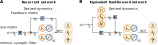
\includegraphics{media/chapters/04_temporal_tuning/recurrent_temporal_tuning.pdf}
	\caption[Solving for some desired temporal tuning in a recurrent neural network]{Solving for some desired temporal tuning in a recurrent neural network. \textbf{(A)} Overview of the recurrent neural network. We need to solve for an input matrix $\mat A$ and a feedback matrix $\mat B$ that realise the desired dynamics for the given intrinsic synaptic filter.
	\textbf{(B)} Assuming that the desired dynamics have already been realised, we obtain a feed-forward network.
	Solving for weight matrices is now a simple least-squares problem.
	Note that the placement of the weight matrices $\mat A$, $\mat B$ and the synaptic filters can be swapped because of linearity.
	}
	\label{fig:recurrent_temporal_tuning}
\end{figure}

Notably, this assumption effectively turns the system into a feed-forward network, which greatly simplifies solving for recurrent weights (cf.~\Cref{fig:recurrent_temporal_tuning}).
In the special case of linear networks, solving for weights directly results in input and feedback matrices $\mat B'$, $\mat A'$.
For first-order synapses these matrices are equal to those returned by the \NEF dynamics principle.

\begin{restatable}{theorem}{thmTemporalLstsq}
	\label{thm:temporal_lstsq}
	Let $\mat A \in \mathbb{R}^{n \times n}$, $\mat B \in \mathbb{R}^{n \times m}$ (w.l.o.g. $m = 1$) represent an \LTI system, $\mathfrak{e}_i$ be the impulse response of its $i$th state dimension, and $h(t)$ be the impulse response of a first-order low-pass:
	\begin{align*}
		  \dot{\vec m}(t) &= \mat A \vec m(t) + \mat B \vec u(t)  \,, 
		& \mathfrak{e}_i(t) &= \big(\!\exp( \mat A t ) \mat B \big)_i \,,
		& h(t) &= \tau^{-1} e^{-t \tau^{-1}} \,.
	\end{align*}
	Let $\mathfrak{x}_k : \mathbb{R}^- \to \mathbb{R}$ be one of $N \geq n + 1$ arbitrary (with some mild constraints; see proof) input signals.
	If all $\mathfrak{e}_i$ and $\mathfrak{x}_k$ are pairwise linearly independent, the following least-squares loss has a unique minimum at $(b'_{i}, a'_{i, 1}, \ldots, a'_{in}) = ( \mat B', \mat A' )_i$ for all $i \in \{1, \ldots, n\}$, where $\mat A' = \tau \mat A + \mat I$, $\mat B' = \tau \mat B$:
	\begin{align*}
		E &=\sum_{k = 1}^{N} \left(
					\int_{0}^{\infty} \!\! \mathfrak{e}_i(\tau) \mathfrak{x}_k(-\tau)
		          - b'_{i} h(\tau) \mathfrak{x}_k(-\tau)
		          - \sum_{j=1}^n a'_{ij} h(\tau) \int_0^\infty \!\! \mathfrak{x}_k(-\tau - \tau') \mathfrak{e}_j(\tau') \, \mathrm{d}\tau' \mathrm{d}\tau \right)^2 \,.
	\end{align*}
\end{restatable}
\noindent This loss function is equal to \cref{eqn:weight_optimise_currents_temporal_no_trafo} in the case of a linear network with $n$ neurons that recurrently connect to themselves, and a \enquote{zeroth} pre-neuron with no temporal tuning providing the input, i.e., $a_0(t) = \mathfrak{x}_k(t)$.
We provide a proof for this in \Cref{app:lstsq_nef_equivalence}.
Similarly, as we discuss in \Cref{app:temporal_tuning_nonlinear}, we can use temporal tuning curves to obtain the same results as the \NEF in the case of nonlinear dynamics and neurons.
Temporal tuning curves are a \emph{generalisation} of the \NEF dynamics principle.

\begin{figure}[p]
	\centering
	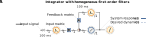
\includegraphics{media/chapters/04_temporal_tuning/recurrence_examples_a_diagram.pdf}\\[0.5em]
	\includegraphics{media/chapters/04_temporal_tuning/recurrence_examples_a.pdf}\\[1em]
	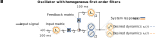
\includegraphics{media/chapters/04_temporal_tuning/recurrence_examples_b_diagram.pdf}\\[0.5em]
	\includegraphics{media/chapters/04_temporal_tuning/recurrence_examples_b.pdf}%
	{\phantomsubcaption\label{fig:recurrence_examples_1a}}%
	{\phantomsubcaption\label{fig:recurrence_examples_1b}}%
	\caption[Realising LTI systems using temporal tuning curves]{
		Realising \LTI systems using temporal tuning curves.
		The depicted networks possess homogeneous first-order low-pass filters as synaptic filters.
		The computed matrices $\mat A$, $\mat B$ are equal to the matrices obtained using the \NEF dynamics principle down to two decimal places.
		We use $N = 1000$ input signals $\mathfrak{x}_k$ of length $T = \SI{10}{\second}$ sampled at $\Delta t = \SI{1}{\milli\second}$ consisting of white noise filtered with a second-order low-pass filter (time-constant $\vartheta = \SI{100}{\milli\second}$).
		Error values $E$ are the \NRMSE.
		\textbf{(A)} Realising an integrator (step impulse-response).
		Note that the system settles at a value slightly smaller than one for a unit pulse input (\emph{left}) due to the aforementioned imprecisions. For a white-noise input (\emph{right}) the result is effectively indistinguishable from the ground-truth solution.
		\textbf{(B)}~Realising a harmonic oscillator by solving for the impulse response of the two-state variables.
		Again, the solution is slightly imprecise causing a small frequency shift.
		In addition, in the case of the unit pulse input (\emph{left}), the system slowly diverges.
	}
	\label{fig:recurrence_examples_1}
\end{figure}

Examples of \LTI systems realised by solving the least-squares loss are depicted in \Cref{fig:recurrence_examples_1}.
Note that there are some minor discrepancies between the numerical and the ideal solution (error is on the order of $10^{-3}$).
These errors are mostly due to time-discretisation at $\Delta t = \SI{1}{\milli\second}$, and would be less noticeable for exponentially decaying impulse responses $\mathfrak{e}_i$.

\newpage

\subsection{Realising LTI Systems in Networks with Complex Recurrence}
\label{sec:lti_complex_networks}

Admittedly, the results presented in the previous subsection are slightly underwhelming.
Solving for the dynamics numerically is computationally expensive,%
\footnote{On the order of one second per processor core, neuron and synaptic filter for $N = {1000}$, $T = \SI{1}{\second}$, $\Delta t = \SI{1}{\milli\second}$.}
and the resulting matrices $\mat A$, $\mat B$ are only precise to about two decimal places (i.e.,~an error of about $10^{-3}$).
%We could obtain better results by just using the closed-form solution.

Still, there are two reasons why our approach is useful.
First, the imprecisions are negligible compared to those resulting from implementing a linear transformation in a spiking neural network.%
\footnote{For $n \approx 100$ neurons, errors due to noise are on the order of $10^{-2}$, whereas errors due to static distortion are on the order of~$10^{-3}$ \citep[cf.][Section~2.2.2 and Figure~2.6, note the squared errors]{eliasmith2003neural}.}
Second, and most importantly, the strength of our approach lies in being agnostic to the network architecture; we can approximate connection weights for networks with higher-order and heterogeneous synaptic filters in the feedback and input paths.

\begin{figure}[p]
	\centering
	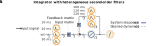
\includegraphics{media/chapters/04_temporal_tuning/recurrence_examples_c_diagram.pdf}\\[0.5em]
	\includegraphics{media/chapters/04_temporal_tuning/recurrence_examples_c.pdf}\\[1.45em]
	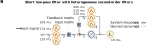
\includegraphics{media/chapters/04_temporal_tuning/recurrence_examples_d_diagram.pdf}\\[0.5em]
	\includegraphics{media/chapters/04_temporal_tuning/recurrence_examples_d.pdf}
	{\phantomsubcaption\label{fig:recurrence_examples_2a}}%
	{\phantomsubcaption\label{fig:recurrence_examples_2b}}%
	\caption[Realising LTI systems in networks with heterogeneous second-order filters]{Realising \LTI systems in networks with heterogeneous second-order filters.
	The depicted networks possess a single linear neuron with multiple heterogeneous synaptic filters.
	The grey line corresponds to a reference solution obtained with a single second-order filter in each path.
	Same setup and legend as described in \Cref{fig:recurrence_examples_1}.
	\textbf{(A)} Implementing an integrator; the pre-synaptic time-constants are much shorter than the post-synaptic time-constants.
	Using \cref{eqn:weight_optimise_currents_temporal}, it is possible to solve for quite precise integrator dynamics.
	\textbf{(B)} Implementing a first-order low-pass with $\tau = \SI{10}{\milli\second}$ in a network with much longer synaptic filters.
	While the response to band-limited white noise (\emph{right}) is reasonably good, there are severe ringing artefacts at input transients, e.g., in the unit pulse (\emph{left}).
	}
	\label{fig:recurrence_examples_2}
\end{figure}

\begin{figure}
	\centering
	\includegraphics{media/chapters/04_temporal_tuning/heterogeneous_recurrence_exploration.pdf}
	\caption[Approximation errors in heterogeneous networks with second-order synaptic filters]{Approximation errors in heterogeneous networks with second-order synaptic filters.
	Errors are the median \NRMSE between the actual and desired response for bandlimited white-noise input over $1000$ trials.
	Dotted orange lines correspond to feed-forward networks; blue lines to recurrent networks.
	See \Cref{fig:recurrence_examples_2} for the architecture and the minimum/maximum filter time-constants in each path.
	Dashed line is a reference network with homogeneous first-order filters ($\tau = \SI{100}{\milli\second}$).
	Shaded areas are the $25$th and $75$percentiles.
	Same training procedure as in \Cref{fig:recurrence_examples_1}; training signals $\mathfrak{x}_k$ are white noise filtered with a second-order low-pass filter with time-constant \SI{100}{\milli\second}.
	\textbf{(A)}~Implementing an integrator.
	Recurrence is required to implement the integrator.
	\textbf{(B)}~Emulating a $\SI{10}{\milli\second}$ first-order low-pass requires recurrence and two or more filters per path (data for two and three filters are equal).
	}
	\label{fig:heterogeneous_recurrence_exploration}
\end{figure}

\subsubsection{Realising integrators and low-pass filters in heterogeneous networks}
To demonstrate this, we next analyse networks with second-order synaptic filters (cf.~\Cref{sec:synaptic_transmission}; eq.~\ref{eqn:low_pass_second_order}) and long, heterogeneous time-constants $\tau$.
Results are depicted in \Cref{fig:recurrence_examples_2,fig:heterogeneous_recurrence_exploration}.
%\begin{align}
%	h(t) &= \frac{t^n}{n! \tau^{n + 1}}  e^{-\frac{t}{\tau}} \,, & H(s) &= \frac{1}{(1 + \tau s)^{n + 1}} \,, & \text{where } n = 1 \text{ results in a second-order filter} \,.
%\end{align}
Our goal is to implement an integrator and a short first-order low-pass filter with $\tau = \SI{10}{\milli\second}$.
Importantly, being able to realise these systems implies that we can implement any \LTI system.%
\footnote{This follows from the controllable canonical form \citep[cf.][Section~3.4.4]{verhaegen2007filtering}, which can be interpreted as chain of leaky integrators (i.e., low-pass filters).}

As is depicted in \Cref{fig:heterogeneous_recurrence_exploration}, the system performance critically depends on placing \emph{multiple} filters with different time-constants in the input and feedback path.%
\footnote{Multiple synaptic filters per connection are technically not compatible with the way our optimisation problem is phrased in \cref{eqn:weight_optimise_currents_temporal}.
However, we can assume that the different feed-forward filters correspond to diverse temporal tuning of different pre-population neurons, and the different recurrent filters are obtained by simply splitting our single neuron into three with the same desired temporal tuning.}
Curiously, this is \emph{more} biologically plausible, since there typically is some variance in synaptic time-constants in biology \citep{jones2014neurotransmitter}.
For the integrator, increasing the number of filters reduces the error by up to two orders of magnitudes, well below what could be realised in a spiking neural network for input bandwidths up to \SI{100}{\hertz}.
The \enquote{short low-pass} system only performs well for input frequencies up to \SI{10}{\hertz}, but similarly requires at least two filters per path.

The necessity for multiple filters follows from \citet[Section~4.4, p.~591]{voelker2018improving}.
To realise a dynamical system with an $n$th order synaptic filter, we must generally provide the first $n - 1$ time-dervatives of the input to the network, i.e., $\mathrm{d} / \mathrm{d} t \, \mathfrak{x}$, $\ldots$, $\mathrm{d} / \mathrm{d} t^{n - 1} \, \mathfrak{x}$.
Accounting for heterogeneous filters similarly requires access to the derivative (cf.~\Cref{app:heterogenous_time_constants}).

The different filters in the feed-forward path can be thought of as being linearly combined to \emph{approximate} these differentials, akin to the \enquote{dual-time-constant networks} explored by \citet{tripp2010population}.
Numerically solving the weight optimisation problem in \cref{eqn:weight_optimise_currents_temporal} automatically determines the weights that implicitly decode the differentials and that, at the same time, \emph{approximate} the desired dynamics.

\begin{figure}
	\centering
	\includegraphics{media/chapters/04_temporal_tuning/heterogeneous_recurrence_exploration_xs_flt.pdf}
	\caption[Effect of the training signal distribution on the system error]{Effect of the training signal distribution on the system error.
	Same setup as in \Cref{fig:heterogeneous_recurrence_exploration}, but for a recurrent network with three filters and with training signals $\mathfrak{x}_k$ of varying bandwidth.
	Training data are generated by low-pass filtering white noise with a second-order low-pass; the time-constant $\rho$ of that filter corresponds to the different line colours (dark blue corresponds high-bandwidth signals, orange to low-frequency signals).
	Data is the median over $1000$ trials, shaded areas are the $25$th and $75$th percentile.
	\textbf{(A)}~For the integrator, there is a trade-off between lower errors in a small frequency range, and larger, but consistent errors  over a larger frequency range.
	\textbf{(B)}~The training distribution has a smaller effect on this network; the optimal solution is mostly independent of the training data.
	}
	\label{fig:heterogeneous_recurrence_exploration_xs_flt}
\end{figure}

\subsubsection{Impact of the training samples $\mathfrak{x}_k$}
The emphasis on \enquote{approximate} is important here.
In contrast to the heterogeneous networks with first-order synaptic filters discussed in the context of \Cref{thm:temporal_lstsq}, there are no guarantees that the final network dynamics are \emph{exactly} the desired dynamics.
Moreover, the ability of the network to generalise depends on the input signals $\mathfrak{x}_k$ used for training.
While this is the norm in most machine learning scenarios, the network in \Cref{thm:temporal_lstsq} did not have this constraint (cf.~\Cref{app:temporal_tuning_proofs}).

We explore the effect of the training signals on the final network in \Cref{fig:heterogeneous_recurrence_exploration_xs_flt}.
Specifically, we generate $\mathfrak{x}_k$ with different frequency content by varying the time-constant $\rho$ of the second-order low-pass filter that is applied to the generated white noise.
Unsurprisingly, only supplying low-frequency inputs (i.e., using a large $\rho$) results in networks that achieve low errors for low-frequency inputs.
A more wide-band input (i.e., using a small $\rho$) results in a compromise-solution with smaller errors for wide-band inputs, but (at least in the case of the integrator) slightly higher errors for low-frequency inputs.

\subsubsection{Relationship to system identification}
When solving for weights in a recurrent system using \cref{eqn:weight_optimise_currents_temporal}, we do not have any formal guarantee that the resulting system is stable---that is, unless the desired dynamics are stable and can be approximated \emph{precisely}.
While, judging from our experience, exponentially decaying temporal tuning curves $\mathfrak{e}_i(t)$ result in stable networks, it would be good to be able to characterise this more thoroughly.

While we are still working on a more thorough analysis, we can at least draw some interesting parallels to the problem of least-squares system identification \citep[cf.][specifically Chapters~7-10]{verhaegen2007filtering}.
That is, we can treat the desired dynamics $\mathfrak{e}_i$ as if they were the output of a black-box system in response to our input signals $\vec{\mathfrak{x}}_k$.
Our goal is to find model parameters $w_{ij}$ that predict the observed output.%
\footnote{Our specific system identification problem is less complex than a general problem.
We directly measure the state, and we do not have instantaneous impulse responses.
Put differently, the output matrix $\mat C$ of our \LTI system is the identity, and the feedthrough matrix $\mat D$ is zero.}

In fact, our optimisation problem in \cref{eqn:weight_optimise_currents_temporal} is a variant of the \enquote{integral-equation approach to system identification} presented by \citet{whitfield1987integralequation}, and, in less developed form, by \citet{squire1971simple}.
The primary difference to our approach is that our networks do not contain perfect integrators---correspondingly, we convolve with the synaptic filter instead of integrating.
This is possible because the integral-equation approach is---at least if the system can be perfectly realised---invariant to convolution with a non-zero filter.

A central challenge of the integral-equation approach is robustness to noise in the measurements, which---even in the case of zero-mean white noise---causes asymptotic biases in the resulting system \citep{sagara1989recursive}.
That is, even as the number of samples $N$ goes to infinity, the estimated system parameters differ from the true system parameters.
Given that we mostly work with artificially generated data, the primary source of noise is time-discretisation.
It may be possible to incorporate more modern weight solving approaches with imposed stability guaranties, as is discussed in \citet{verhaegen2007filtering}.

\subsubsection{Realising dynamics in recurrences with intermediate populations}

\begin{figure}
	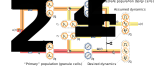
\includegraphics{media/chapters/04_temporal_tuning/recurrent_network_intermediate.pdf}
	\caption[Approximating dynamical systems across intermediate populations]{Approximating dynamical systems across intermediate populations. Both neuron populations receive input $u(t)$ through a set of synaptic filters with time-constants $\tau_1$, $\tau_4$; the upper, or \enquote{intermediate} population then projects onto the lower population, the lower population provides the output and projects onto the upper population. Each feedback path passes through another set of filters with time-constant $\tau_2$, $\tau_3$.
	As before, we can solve for connection weights $\mat A_1'$, $\mat A_2'$, $\mat B_1'$, $\mat B_2'$ by assuming that the desired dynamics have already been realised (scissor symbol and dotted lines).
	We must then account for all possible paths (coloured backgrounds) from the input $u(t)$ to the output $\vec m(t)$.
	}
	\label{fig:recurrent_network_intermediate}
\end{figure}

So far, we assumed that recurrent connections are tight loops that originate in a certain population and laterally target neurons in the same population.
This is not necessarily the case in biology.
As we mentioned in the context of Dale's principle in \Cref{sec:nef_limitations,sec:nef_nonneg}, inhibitory input passes through interneuron populations.
Fortunately, the interneurons typically do not dramatically affect the overall network dynamics \citep{parisien2008solving}.

There are, of course, exceptions to this.
As we discuss in more detail in \Cref{chp:cerebellum}, the Granule-Golgi microcircuit in the cerebellum possesses relatively slow synapses in the connection from the excitatory granule cells to the inhibitory Golgi cells.%
\footnote{As reported by \citet{dieudonne1998submillisecond}, the synaptic dynamics of the granule to Golgi projection can be modelled using second order filter dynamics and time-constants of $\tau_1 \approx \SI{31}{\milli\second}$ and $\tau_2 \approx \SI{170}{\milli\second}$ (cf.~eq.~\ref{eqn:low_pass_second_order}); this corresponds to a first-order low-pass filter with a time-constant of about \SIrange{60}{70}{\milli\second}.}
Additionally, the interneurons receive the same input $u(t)$ as the excitatory population \citep{dangelo2013cerebellar}, which does not fit our canonical picture of interneuron populations.

\Cref{fig:recurrent_network_intermediate} illustrates this \enquote{Granule-Golgi circuit} schematically.
To realise an \LTI system $\mat A$, $\mat B$ in such a circuit, we must find weight matrices $\mat A_1'$, $\mat A_2'$, $\mat B_1'$, $\mat B_2'$ that compensate for the network dynamics.
We next discuss two ways to approach this problem.

\begin{figure}
	\includegraphics{media/chapters/04_temporal_tuning/recurrence_example_intermediate.pdf}
	\caption[Realising an integrator in a recurrent network with an intermediate population]{Realising an integrator in a recurrent network with an intermediate population and heterogeneous synaptic filters. Same experimental setup as in \Cref{fig:recurrence_examples_1}; errors $E$ are the \NRMSE.
	\textbf{(A)}~A single filter per path ($\tau_1 = \tau_4 = \SI{10}{\milli\second}$, $\tau_2 = \tau_3 = \SI{100}{\milli\second}$).
	Errors are relatively large, since we do not compensate for the second-order filter formed by the filter-chain.
	\textbf{(B)} Placing three filters in each path (for a total of $21$ weights) results in smaller errors (time-constants are between \SIrange{10}{30}{\milli\second} in the input path, and \SIrange{100}{120}{\milli\second} in the recurrent path).
	We sidestep splitting the computed weight matrices by simulating a partially collapsed network; this has no influence on the network function.
	}
	\label{fig:recurrence_example_intermediate}
\end{figure}

\paragraph{Ascribing temporal tuning to the interneuron population}
First, we could simply decide on some temporal tuning for the interneuron population and use \cref{eqn:weight_optimise_currents_temporal} to solve for connection weights.
If both neuron populations possess the same temporal tuning, then the interneurons appear as a pass-through to the primary population.
Assuming homogeneous first-order synaptic filters with time-constant $\tau$, the closed-form solution is
\begin{align}
	\mat A_1' &= \mat A_2' = \tau \mat A + \mat I \,, & \mat B_1' &= \mat B_2' = \tau \mat B \,.
\end{align}
Put differently, we use the closed-form solution from the \NEF dynamics principle in both paths.
This makes intuitive sense due to symmetry, but see \Cref{app:granule_golgi_dynamics} for a detailed derivation.

\paragraph{Unrolling the network}
An alternative approach is to solve for all weights simultaneously.
Assuming that we have already realised the desired tuning at the output of the network, and because all our neurons and filters are linear (cf.~the beginning of \Cref{sec:temporal_tuning_lti}), we can \enquote{unroll} the network into several feed-forward paths (coloured in \Cref{fig:recurrent_network_intermediate}).

Let $h_1$, $\ldots$, $h_4$ denote the individual synaptic filters.
Furthermore, to simplify our notation, let $\mathfrak{e}$ be a vectorial function $\mathfrak{e} : \mathbb{R}^+ \longrightarrow \mathbb{R}^q$, and let \enquote{$\ast$} denote elementwise convolution.
We obtain the following loss function:
{%
%\newcommand{\pathOne}[1]{\mbox{\colorbox{IndianRed}{$\displaystyle {#1}$}}}%
%\newcommand{\pathTwo}[1]{\mbox{\colorbox{Gold}{$\displaystyle {#1}$}}}%
%\newcommand{\pathThree}[1]{\mbox{\colorbox{YellowGreen}{$\displaystyle {#1}$}}}%
\newcommand{\pathOne}[1]{#1}%
\newcommand{\pathTwo}[1]{#1}%
\newcommand{\pathThree}[1]{#1}%
\begin{align}
	E = \sum_{k = 1}^N \, \bigl\| \, (\mathfrak{x}_k \ast \mathfrak{e})(0)
		- \pathOne{\mat{B}_2' (h_4 \ast u)(0)}
		- \pathTwo{\mat{A}_1' \mat{B}_1' \bigl(h_3 \ast (h_1 \ast u)\bigr)(0)}
		- \pathThree{\mat{A}_1' \mat{A}_2' \bigl(h_3 \ast (h_2 \ast \mathfrak{e})\bigr)(0)}
	\, \bigr\|_2^2 \,.
\end{align}}%
Minimising this loss function results in the matrix products $\mat{A}_1' \mat{A_2}'$ and $\mat{A}_1' \mat{B}_1'$ instead of the individual matrices; however, the weights can be split arbitrarily in a post-processing step.
\Cref{fig:recurrence_example_intermediate} depicts the results of realising an integrator using this method.
